\newthought{\textbf{Taravia Fauzah- 2020903430054 - TRKJ 3B}}

\newday{\textbf{13-20 Oktober 2022} - Instalasi dan Konfigurasi Hadoop}
\begin{enumerate}
\item Kendala dan Solusi
% jelaskan kendala dan penyebab yang dialami saat mengikuti praktikum serta solusi atau langkah-langkah yang telah dilakukan
\newline praktikum pertama yaitu instalasi apache hadoop. selama mengerjakan praktikum mengikuti modul tidak ada kendala

\begin{figure}[!ht]
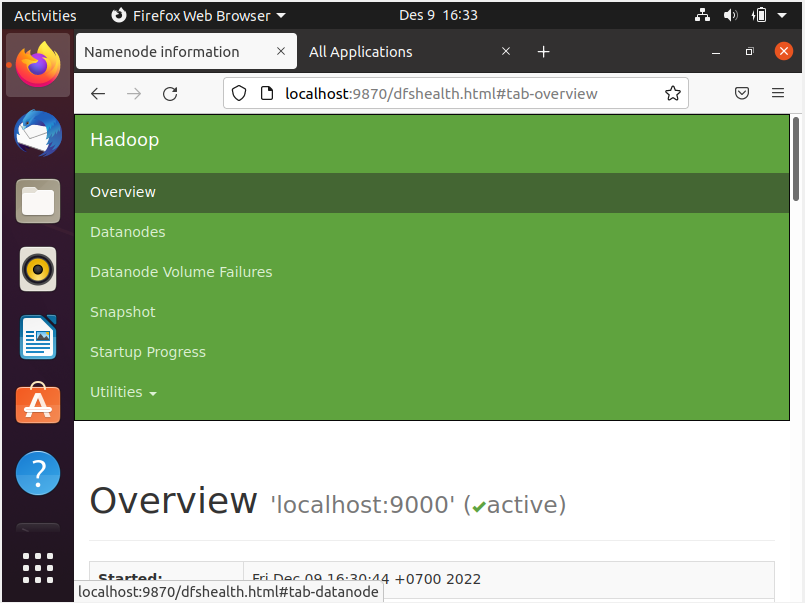
\includegraphics[width=\textwidth]{TaraviaFauzah/akses-localhost-9078}
\caption{hasil dari cek hadoop service}
\label{gam:perkuliahan15-9}
\end{figure}

\begin{figure}[!ht]
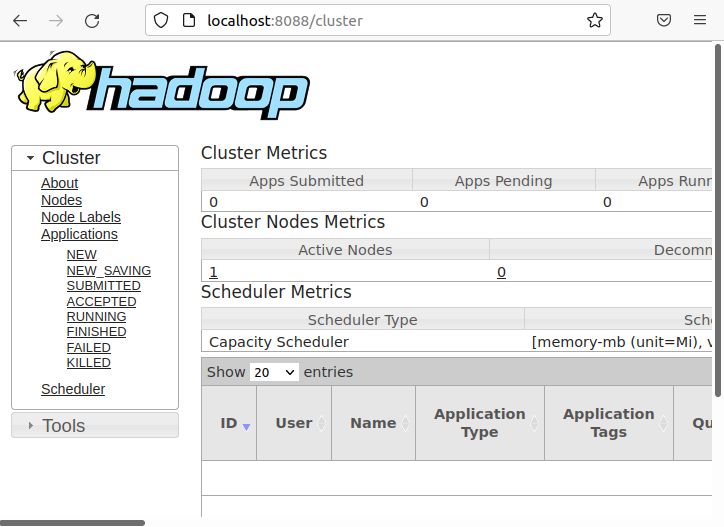
\includegraphics[width=\textwidth]{TaraviaFauzah/akses-localhost-8088}
\caption{hasil dari cek hadoop service}
\label{gam:perkuliahan15-9}
\end{figure}

\item Kesimpulan
% berikan kesimpulan dari praktikum yang telah dikerjkan
\newline Berhasil mendownload dan menginstal Apache hadoop dan sudah bisa di jalankan 
\end{enumerate}

\newday{\textbf{10 November 2022} - WordCount bawaan Hadoop}
\begin{enumerate}
\item Kendala dan Solusi
% jelaskan kendala dan penyebab yang dialami saat mengikuti praktikum serta solusi atau langkah-langkah yang telah dilakukan
\newline pada praktikum kali ini membuat program WordCount Bawaan Hadoop.pada saat praktikum tidak ada kendala hanya saja error karena salah menulis perintah.

\begin{figure}[!ht]
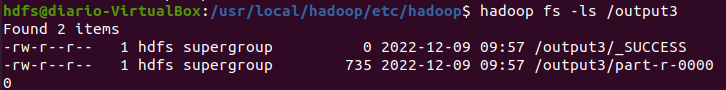
\includegraphics[width=\textwidth]{TaraviaFauzah/output}
\caption{hasil dari hadoop fs}
\label{gam:perkuliahan1-10}
\end{figure}

\begin{figure}[!ht]
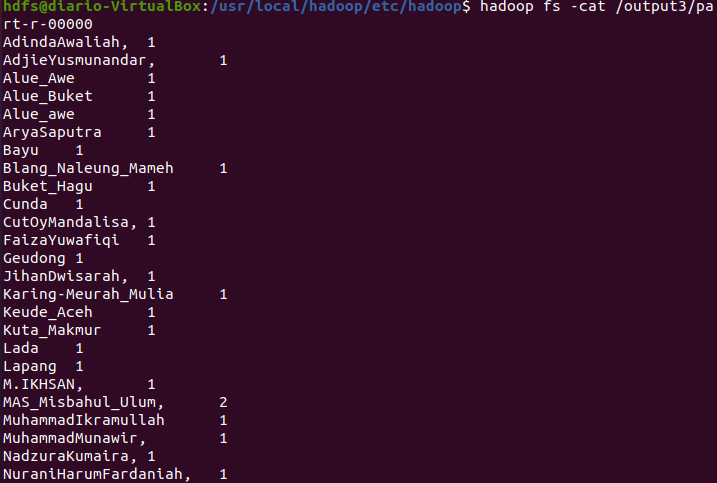
\includegraphics[width=\textwidth]{TaraviaFauzah/output1}
\caption{hasil dari hadoop fs}
\label{gam:perkuliahan1-10}
\end{figure}

\begin{figure}[!ht]
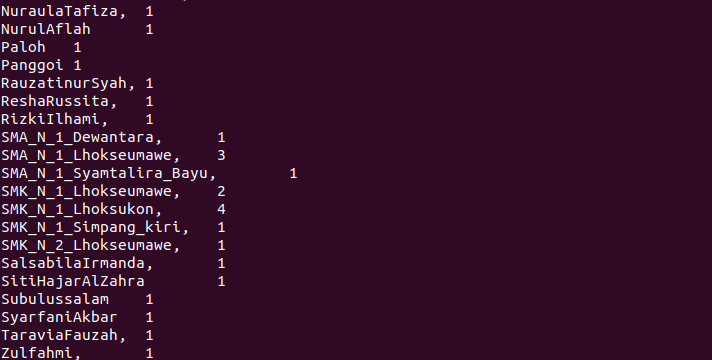
\includegraphics[width=\textwidth]{TaraviaFauzah/output1_1}
\caption{hasil dari hadoop fs}
\label{gam:perkuliahan1-10}
\end{figure}

\item Kesimpulan
% berikan kesimpulan dari praktikum yang telah dikerjkan
\newline langkah praktikum ini adalah untuk memahami proses cara kerja pada hadoop dalam memproses data input sehingga menghasikan sebuah output. wordcount adalah program untuk menghitung jumlah kata dalam inpu.

\end{enumerate}

\newday{\textbf{17 November 2022} - WordCount dengan Java}
\begin{enumerate}
\item Kendala dan Solusi
% jelaskan kendala dan penyebab yang dialami saat mengikuti praktikum serta solusi atau langkah-langkah yang telah dilakukan
\newline pada praktikum kali ini membuat program WordCount dengan java.pada saat praktikum memiliki error tapi errornya di sebabkan tidak teliti saat menulis codingan yang ada di modul.solusinya harus lebih teliti saat mengerjakan codingan tersebut.

\begin{figure}[!ht]
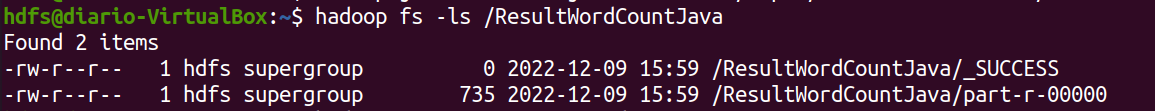
\includegraphics[width=\textwidth]{TaraviaFauzah/hasil1}
\caption{hasil dari hadoop fs WordCount}
\label{gam:perkuliahan2-12}
\end{figure}

\begin{figure}[!ht]
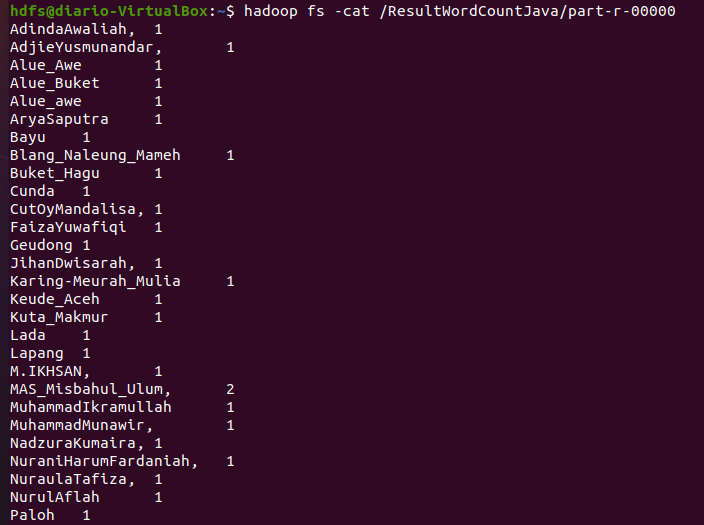
\includegraphics[width=\textwidth]{TaraviaFauzah/hasil2}
\caption{hasil dari hadoop fs WordCount}
\label{gam:perkuliahan2-12}
\end{figure}

\begin{figure}[!ht]
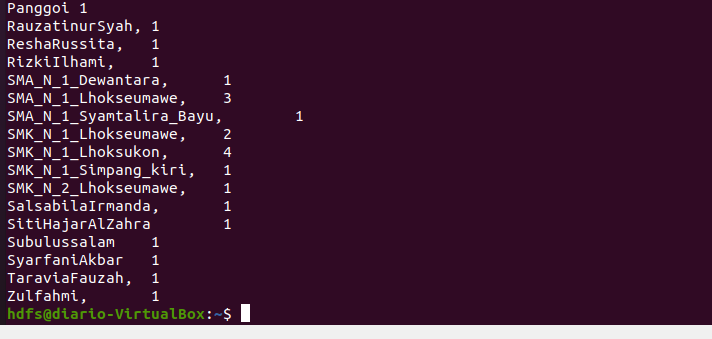
\includegraphics[width=\textwidth]{TaraviaFauzah/hasil2_2}
\caption{hasil dari hadoop fs WordCount}
\label{gam:perkuliahan2-12}
\end{figure}

\item Kesimpulan
% berikan kesimpulan dari praktikum yang telah dikerjkan
\newline berhasil menjalan program WordCount dengan java

\end{enumerate}

\newday{\textbf{24 November 2022} - instalasi apache Spark (Pyspark)}
\begin{enumerate}
\item Kendala dan Solusi
% jelaskan kendala dan penyebab yang dialami saat mengikuti praktikum serta solusi atau langkah-langkah yang telah dilakukan
\newline pada praktikum kali ini instalasi apache spark (pyspark)tidak ada kendala.

\begin{figure}[!ht]
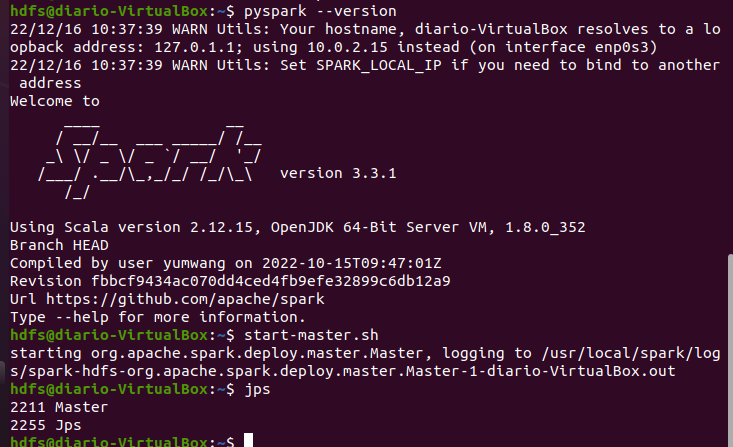
\includegraphics[width=\textwidth]{TaraviaFauzah/pyspark version}
\caption{hasil dari pyspark version}
\label{gam:perkuliahan2-15}
\end{figure}

\item Kesimpulan
% berikan kesimpulan dari praktikum yang telah dikerjkan
\newline berhasil menjalan pyspark yang sudah terinstall.
\end{enumerate}

\newday{\textbf{1 Desember 2022} - Program WordCount dengan Python}
\begin{enumerate}
\item Kendala dan Solusi
\newline pada praktikum kali ini membuat program wordcount dengan python,pada saat mengeisi codingan di nanonya harus lebih teliti supaya tidak terjadi error.

\newpage
\begin{figure}[!ht]
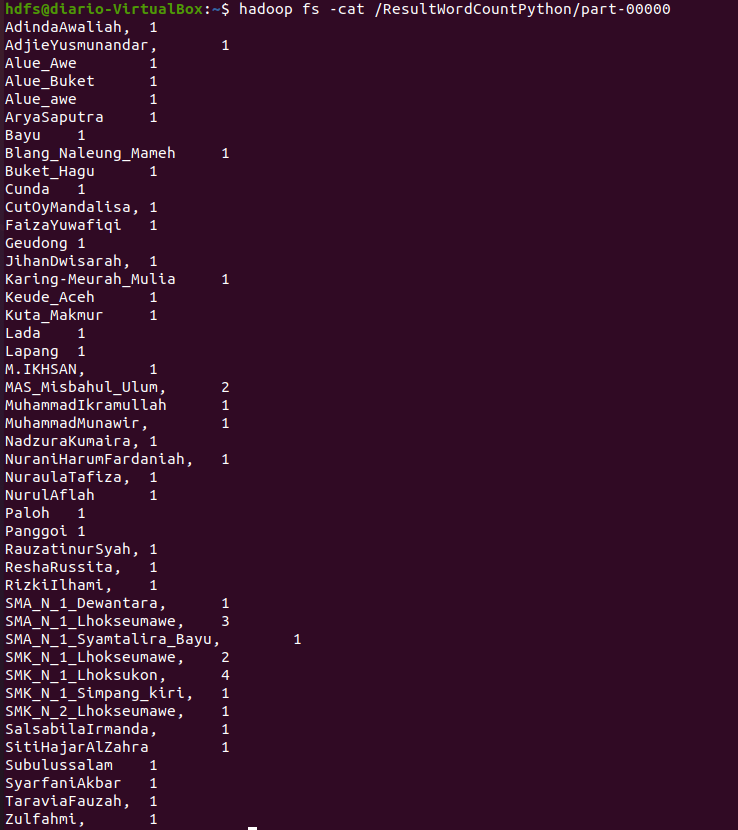
\includegraphics[width=\textwidth]{TaraviaFauzah/hasil WordCountPython2}
\caption{lihat hasil dari WordCountPython }
\label{gam:perkuliahan2-15}
\end{figure}

\begin{figure}[!ht]
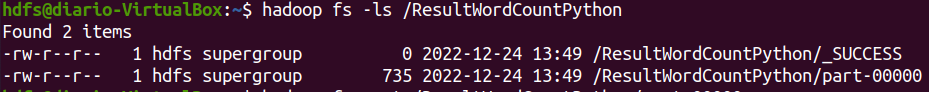
\includegraphics[width=\textwidth]{TaraviaFauzah/hasil WordCounPython1}
\caption{Cek hasil dari WordCountPython }
\label{gam:perkuliahan2-15}
\end{figure}

\item Kesimpulan
\newline berhasil membuat pemograman WordCount dengan Python.
\end{enumerate}

\newday{\textbf{8 Desember 2022} - Program WordCount dengan PySpark}
\begin{enumerate}
\item Kendala dan Solusi
\newline pada praktikum kali ini membuat program wordcount dengan pySpark,pada saat mengeisi codingan di nanonya harus lebih teliti supaya tidak terjadi error.

\begin{figure}[!ht]
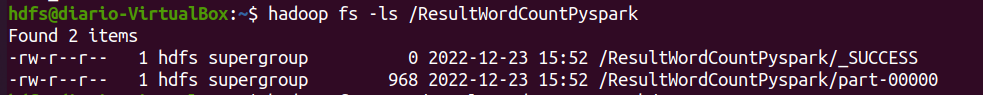
\includegraphics[width=\textwidth]{TaraviaFauzah/hasil WordCountPySpark1}
\caption{cek hasil dari WordCountPySpark }
\label{gam:perkuliahan2-15}
\end{figure}

\newpage
\begin{figure}[!ht]
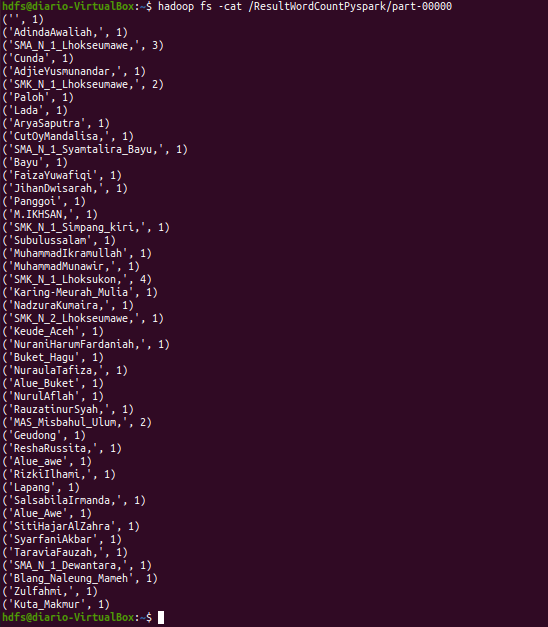
\includegraphics[width=\textwidth]{TaraviaFauzah/hasil WordCountPySpark2}
\caption{lihat hasil dari WordCountPySpark }
\label{gam:perkuliahan2-15}
\end{figure}

\item Kesimpulan
\newline berhasil membuat pemograman WordCount dengan PySpark.
\end{enumerate}

\newday{\textbf{15 Desember 2022}- Tugas Individu}
\begin{enumerate}
\item Kendala dan Solusi
\newline pada pengerjaan tugas individu tidak ada kendala,hanya saja kita harus lebih teliti pada saat mengerjakan program pada terminal pyspark tersebut.
% jelaskan kendala dan penyebab yang dialami saat mengikuti praktikum serta solusi atau langkah-langkah yang telah dilakukan

\begin{figure}[!ht]
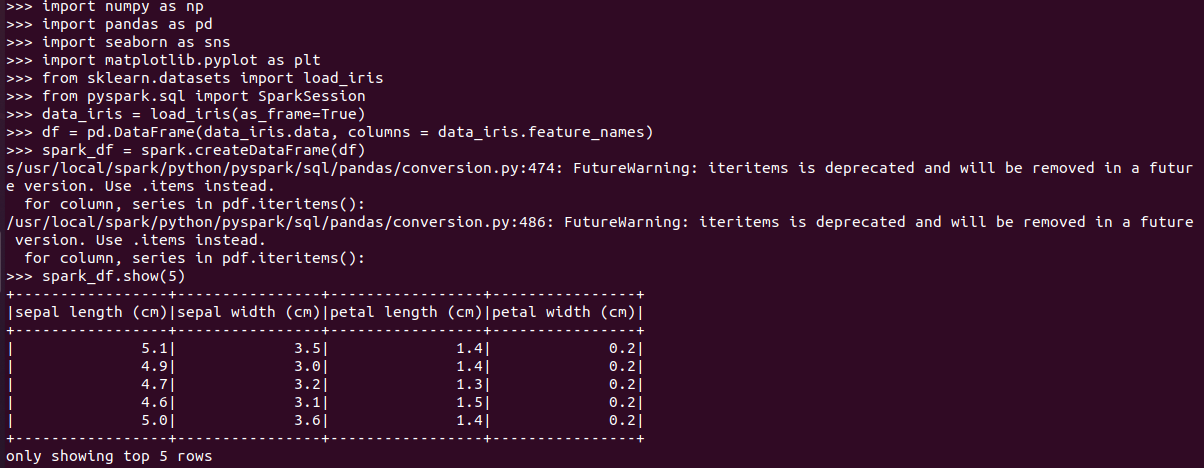
\includegraphics[width=\textwidth]{TaraviaFauzah/load package dan load data}
\caption{codingan pada terminal pyspark untuk load package dan load data dan beserta hasilnya }
\label{gam:perkuliahan2-15}
\end{figure}

\newpage
\begin{figure}[!ht]
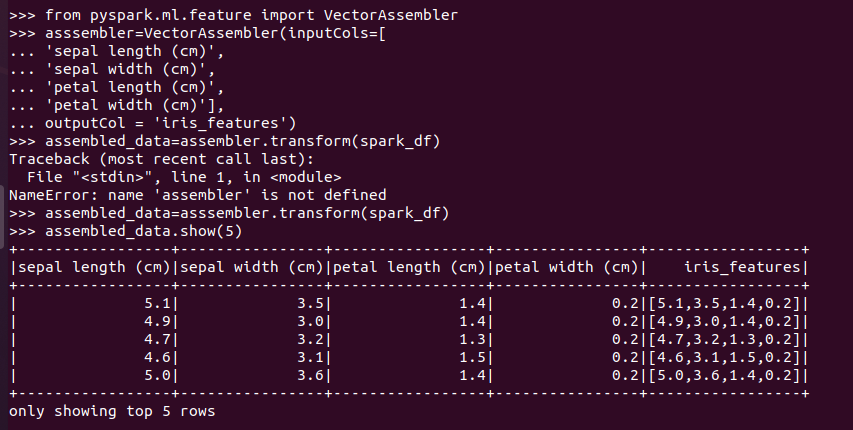
\includegraphics[width=\textwidth]{TaraviaFauzah/import VectorAssembler}
\caption{codingan pada terminal pyspark untuk import VectorAssembler }
\label{gam:perkuliahan2-15}
\end{figure}

\begin{figure}[!ht]
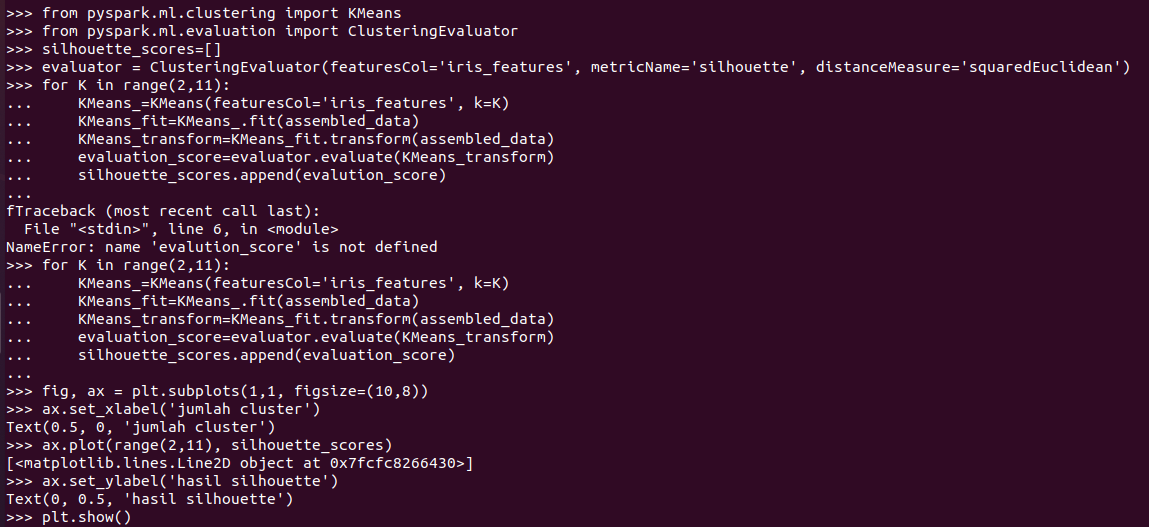
\includegraphics[width=\textwidth]{TaraviaFauzah/import KMeans}
\caption{codingan pada terminal pyspark untuk import KMeans }
\label{gam:perkuliahan2-15}
\end{figure}

\begin{figure}[!ht]
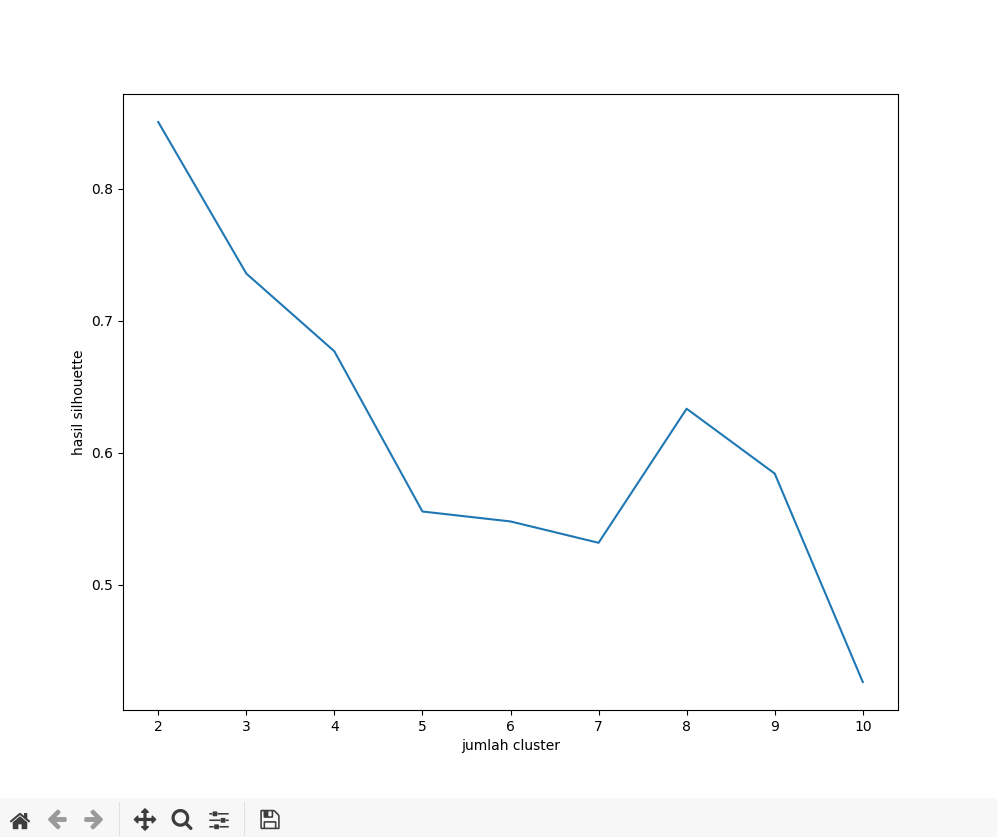
\includegraphics[width=\textwidth]{TaraviaFauzah/hasil import KMeans}
\caption{hasil dari hasil import KMeans }
\label{gam:perkuliahan2-15}
\end{figure}

\newpage
\begin{figure}[!ht]
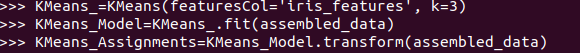
\includegraphics[width=\textwidth]{TaraviaFauzah/model KMeans clustering}
\caption{codingan pada terminal pyspark untuk model KMeans clustering}
\label{gam:perkuliahan2-15}
\end{figure}

\begin{figure}[!ht]
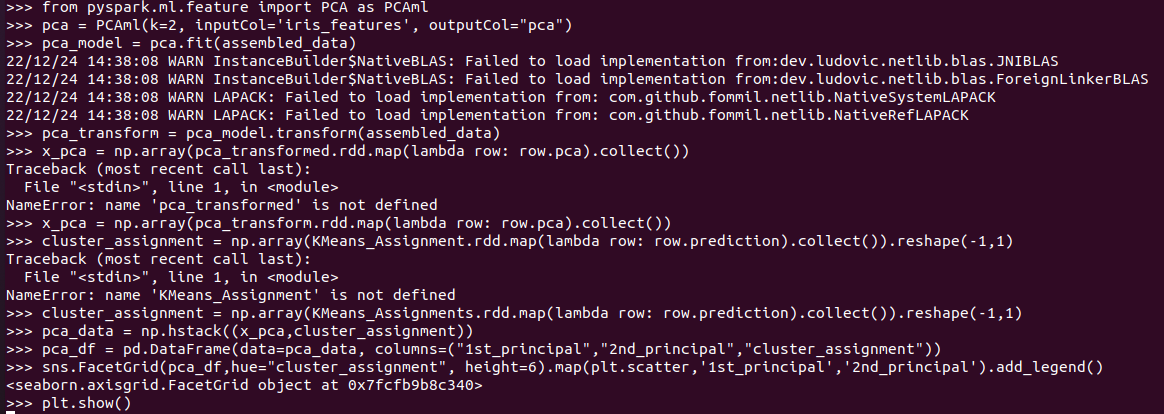
\includegraphics[width=\textwidth]{TaraviaFauzah/clustering dengan PCA}
\caption{codingan pada terminal pyspark untuk clustering dengan PCA}
\label{gam:perkuliahan2-15}
\end{figure}

\begin{figure}[!ht]
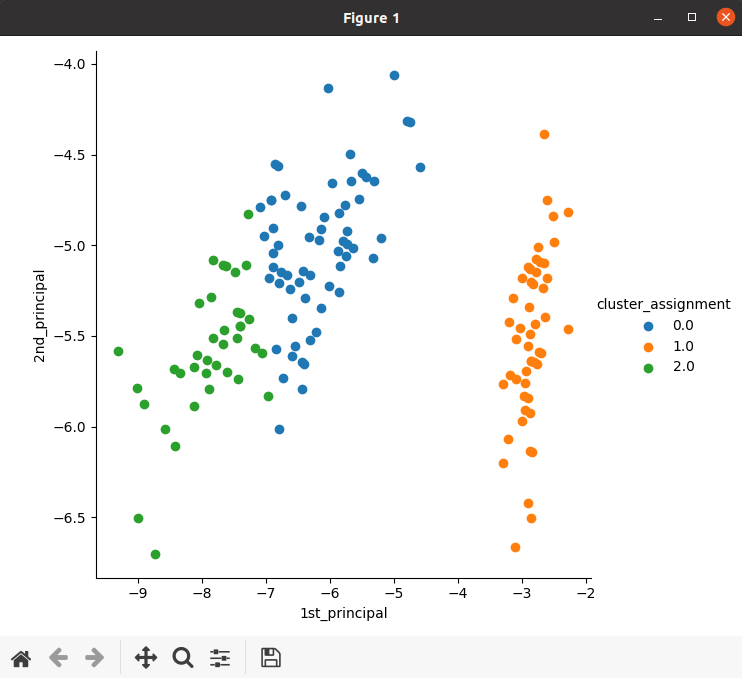
\includegraphics[width=\textwidth]{TaraviaFauzah/hasil clustering dengan PCA}
\caption{hasil dari clustering dengan PCA}
\label{gam:perkuliahan2-15}
\end{figure}

\item Kesimpulan
% berikan kesimpulan dari praktikum yang telah dikerjkan
\newline pada saat pengerjaan tugas tersebut berjalan dengan lancar karena tidak ada error.dan tugas individu berhasil di selesaikan

\end{enumerate}

